%******************************************************************************%
%                                                                              %
%                  sample.en.tex for LaTeX                                     %
%                  Created on : Tue Mar 10 13:27:28 2015                       %
%                  Made by : David "Thor" GIRON <thor@42.fr>                   %
%                                                                              %
%******************************************************************************%

\documentclass{42-en}


%******************************************************************************%
%                                                                              %
%                                    Header                                    %
%                                                                              %
%******************************************************************************%
\begin{document}



                           \title{Structured Query Language: Basics!}
                          \subtitle{The world is a zoo, you've seen the news}
                       \member{Ted Tran}{ttran@student.42.us.org}
                        \member{42 Ghost Bum}{pedago@42.fr}

\summary {
  This project is an introduction to \texttt{SQL} using material 
  from \href{https://sqlzoo.net}{SQLZoo}.
}

\maketitle

\tableofcontents


%******************************************************************************%
%                                                                              %
%                                  Foreword                                    %
%                                                                              %
%******************************************************************************%
\chapter{Foreword}

	You know, at the end of the day, if you're stuck, you can easily get the 
	vast majority of answers using google. SQLBolt and SQLZoo are probably 
	the most popular resources to learn SQL these days. \\
	
	But have no fear! \\ 

	I wrote a \texttt{TON} of extra queries for you all to complete and have fun 
	doing. And by fun, I mean as fun as falling into a gorilla enclosure at a 
	zoo. Prepare for a world of \texttt{hurt} due to one man's good intentions. \\

	Good luck! \\

	If you need help, you won't get it until you go onto the HackHighSchool slack 
	and @(any mentor who's not in charge of the SQL curriculum) 10 times and show me proof. \\

	And remember-- please try solving the problem on your own using your massive brain, 
	Google, or asking your peers before coming to me. \\ 

	I'm sure you're wondering, "Why is this foreword so long?". I'll tell you why, the real truth. 
	It's because the xkcd comic on the page after this one is so long, so I need to put filler 
	text in to fill this page so it doesn't look empty. \\

	You know what? I think you're being ungrateful. Just because of that, I'm going to write 
	the rest of the learning material in French then google translate it into Vietnamese, 
	Spanish, Japanese, and German before English to get the real authenticity of a 42 PDF. \\ 

	But have no fear, High School students! -> Do not worry, student!

    % Spacing in the source code does not influence spacing in the
    % generated pdf. The blank lines aboves and below won't appear.
    % Instead, use \newline (or its shortcut \\) and \newpage to
    % create vertical spacing.
    
            \begin{figure}[H]
                \begin{center}
                    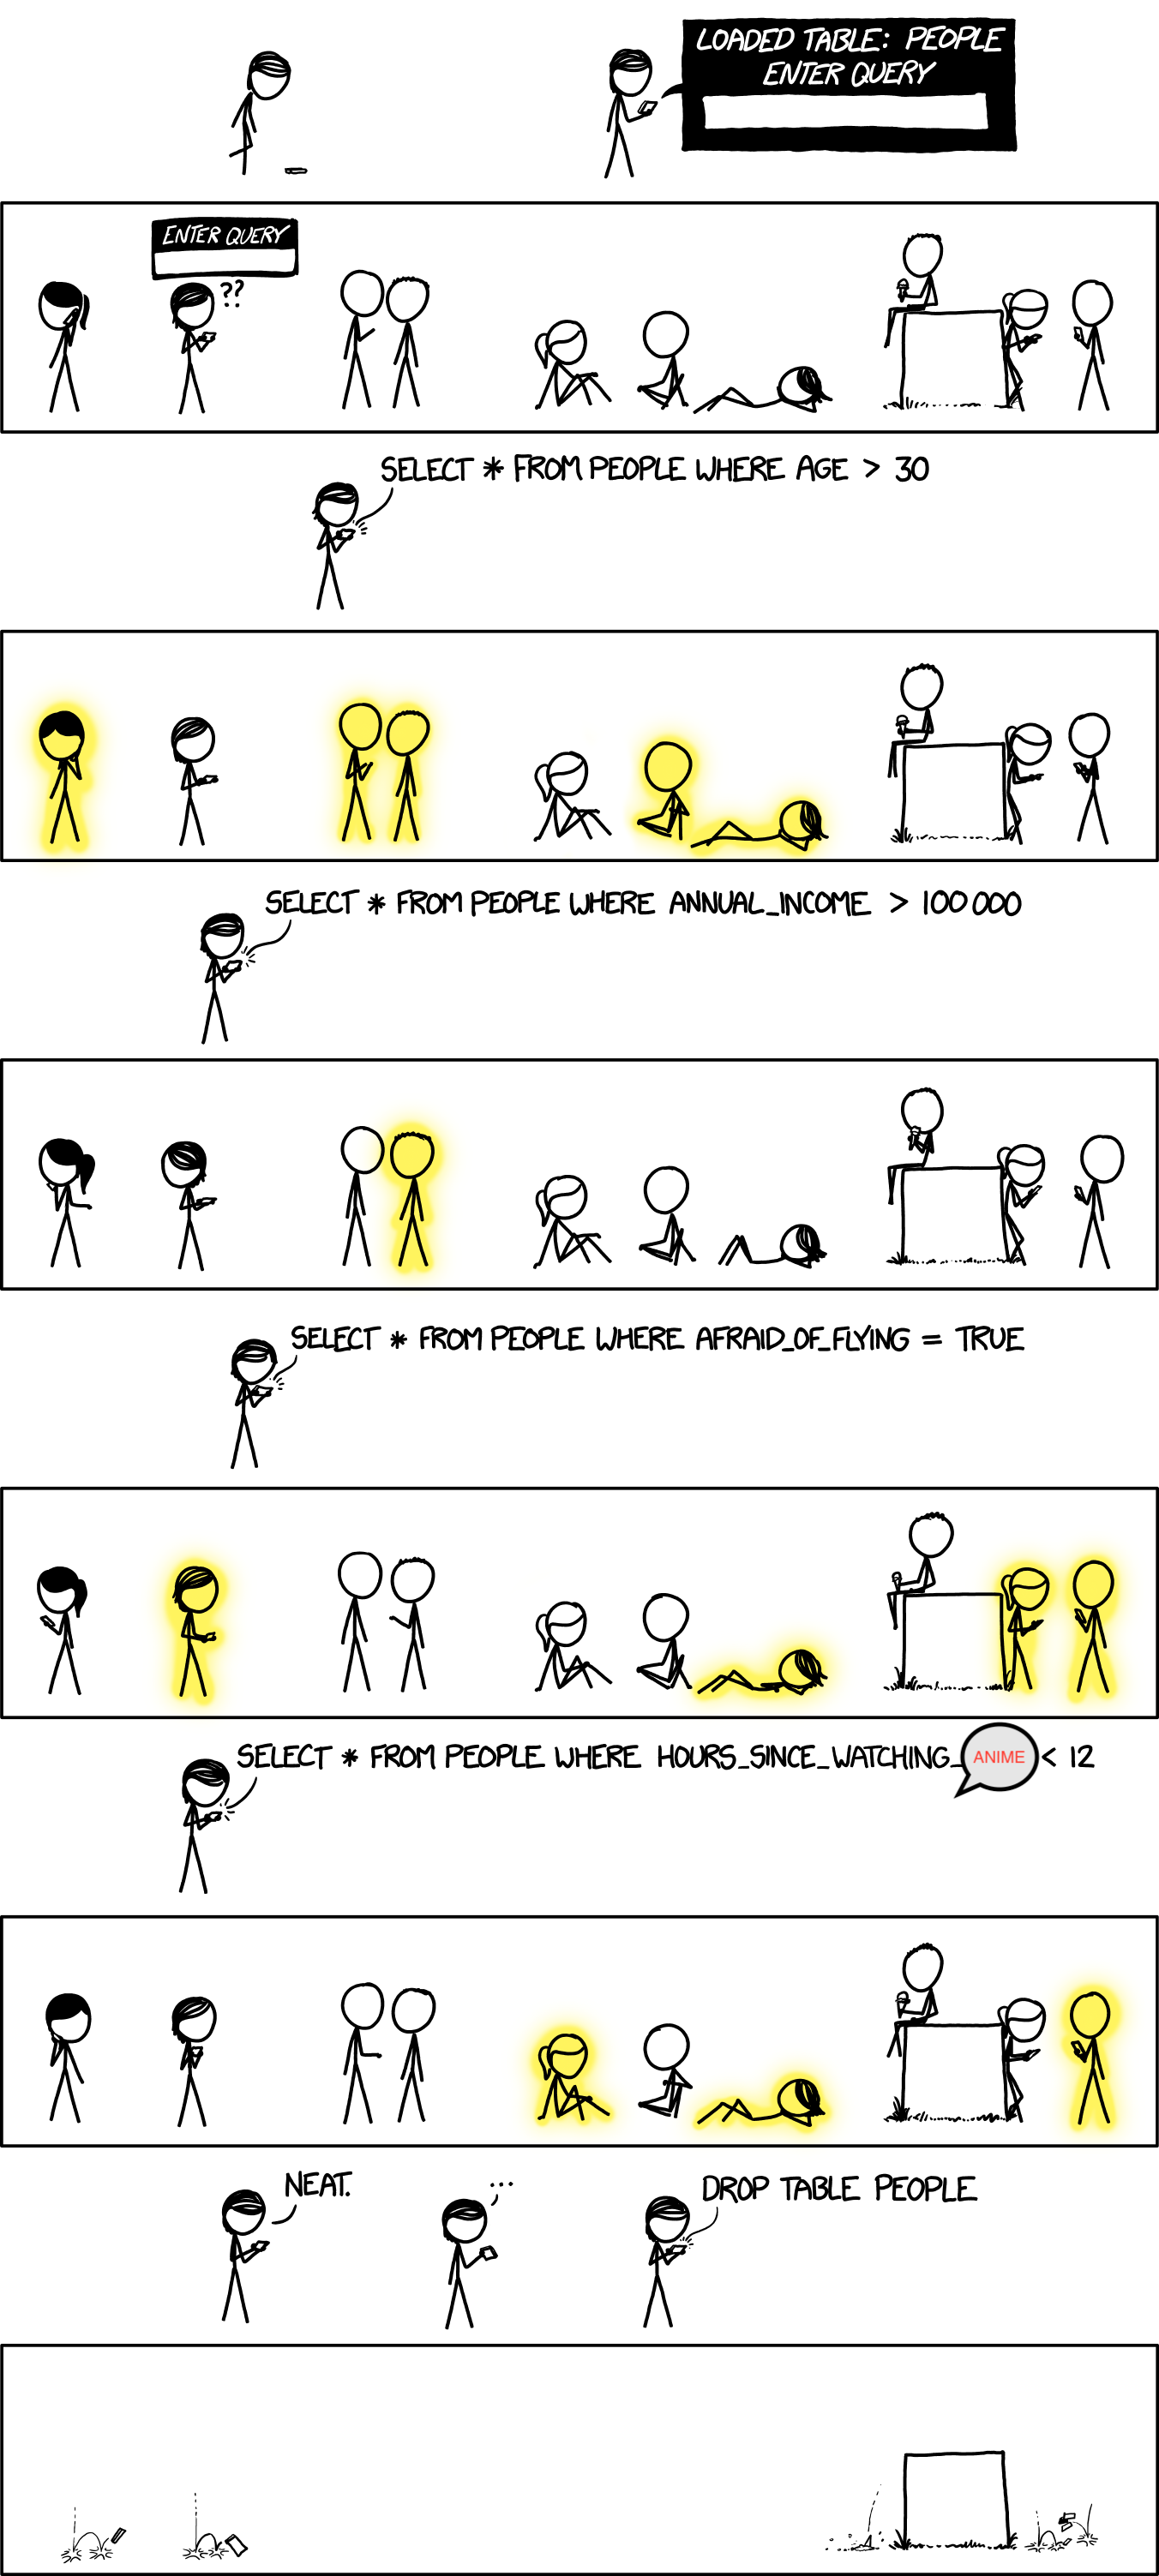
\includegraphics[width=10cm]{query_2x.png}
                \end{center}
            \end{figure}

	    	\newpage 	

%******************************************************************************%
%                                                                              %
%                                 Introduction                                 %
%                                                                              %
%******************************************************************************%
\chapter{Introduction}

	What the hell am I going to be doing?

	\begin{itemize}\itemsep1pt
		\item First, you're going to be running a ton of docker commands 
			so that you can run various things on these 42 lab computers
		\item Next, you're going to be learning all the SQL fundamentals! 
		\item It'll be learning through experience, so be prepared to write 
			a ridiculous amount of queries. 
		\item Once you have the fundamentals down, it'll be time for you to 
			write a wrapper so users can interact with the database 
			without writing any SQL queries(since you wrote em' already!) 
	\end{itemize}


	Testing is provided for you, so you only need to run a single command to 
	check your answers! Go for the green, buddy. 

%******************************************************************************%
%                                                                              %
%                                  Goals                                       %
%                                                                              %
%******************************************************************************%
\chapter{Goals}

	\begin{itemize}\itemsep1pt 
		\item Learn best practices for writing SQL queries   
		\item Learn SQL fundamentals to query the database for required information 
		\item Create a wrapper using a programming language of your choice, so 
			that a person can obtain information from the database without 
			having to write SQL queries themselves.
	\end{itemize}

	Your goal is to pass every single test for a beautiful 100 percent GREEN. Then 
	after that, use what you've learned at H2S to create an interface for users 
	to get what they want from the DB without writing SQL themselves. 

%******************************************************************************%
%                                                                              %
%                             General instructions                             %
%                                                                              %
%******************************************************************************%
\chapter{General instructions}

	\begin{itemize}\itemsep1pt 
		\item This project will be corrected by humans only. 
			You're allowed to organize and name your files as you see 
			fit, but you must follow the following rules. 
		\item The first rule of SQL Club is: You do not talk about SQL Club.
		\item The second rule of SQL Club is: You do not talk about SQL Club.
		\item I was going to copy the third rule from the 42 PDF, "You are never allowed 
			to submit code you did not write yourself" but that'd make me a hypocrite. 
			Go wild!
		\item Within the mandatory part, you are only allowed to use SQL. 
		\item You can ask your questions on slack and random people in your nearby vicinity 
			that appear to be older than you. Of course, with the exception being me-- don't ask me 
			any questions. Everybody at 42 is a SQL master, and H2S mentors are required 
			to have a PhD in Structured Query Language studies! So don't be afraid to 
			come to them for guidance.
		\item You will be provided with instructions on how to setup your programming environment, create the DB 
			and import data, a skeleton to code in, and a full testing suite to check your answers.
	\end{itemize}

% Don't forget this line for piscine days to initate the exercise counter at 0
\startexercices

%******************************************************************************%
%                                                                              %
%                             THE SQL PISCINE LOL                              %
%                                                                              %
%******************************************************************************%

\chapter{Day \exercicenumber: Beginning your SQL studies! }

\extitle{SQL SELECT/FROM/WHERE, operators, DISTINCT, expression aliases, *}
\exfiles{01\_select.rb, 02\_select.rb, 03\_select.rb, 03a\_select.rb}
\exnotes{Make sure to use docker cp to store your files on the host computer, then add it to a git repo after!}
\makeheaderfiles

	Look at this example! \\
    
            \begin{figure}[H]
                \begin{center}
                    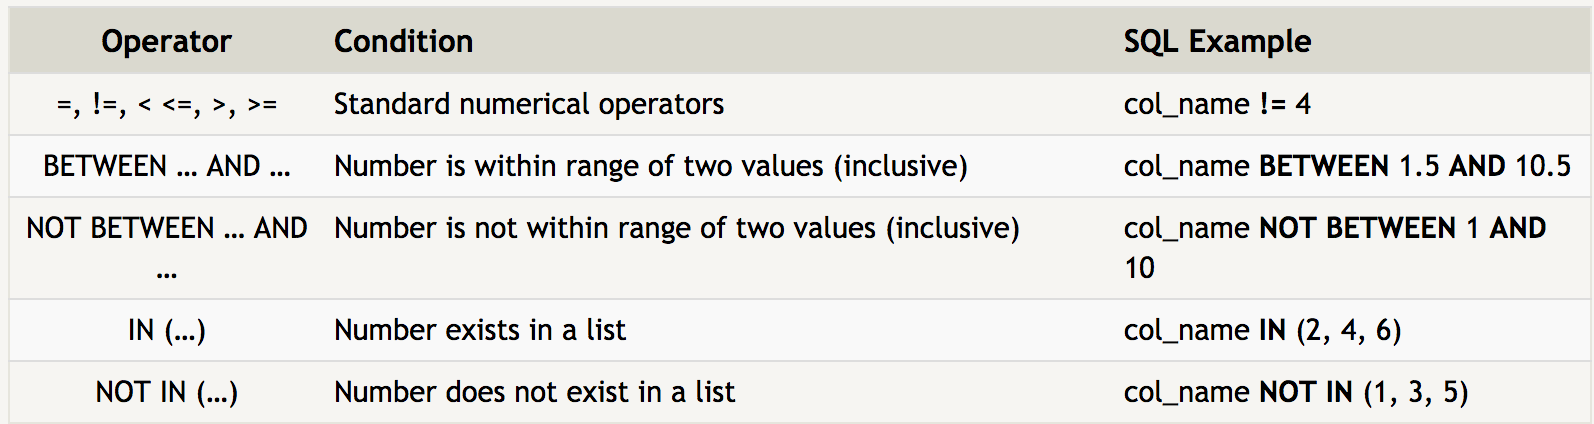
\includegraphics[width=14cm]{operators.png}
                \end{center}
            \end{figure}

	\begin{itemize}\itemsep1pt 
		\item SELECT chooses which columns to grab 
		\item FROM chooses which table to start from
		\item DISTINCT means you want this to be unique! No duplicates 
		\item * basically means that  you'll grab ALL. 
		\item You can aliases expressions or tables using "AS", this keeps your SQL code DRY. 
		\item WHERE is used to filter records by condition! 
		\item Now, what are some useful operators you can use in the WHERE clause?  
	\end{itemize}

    
            \begin{figure}[H]
                \begin{center}
                    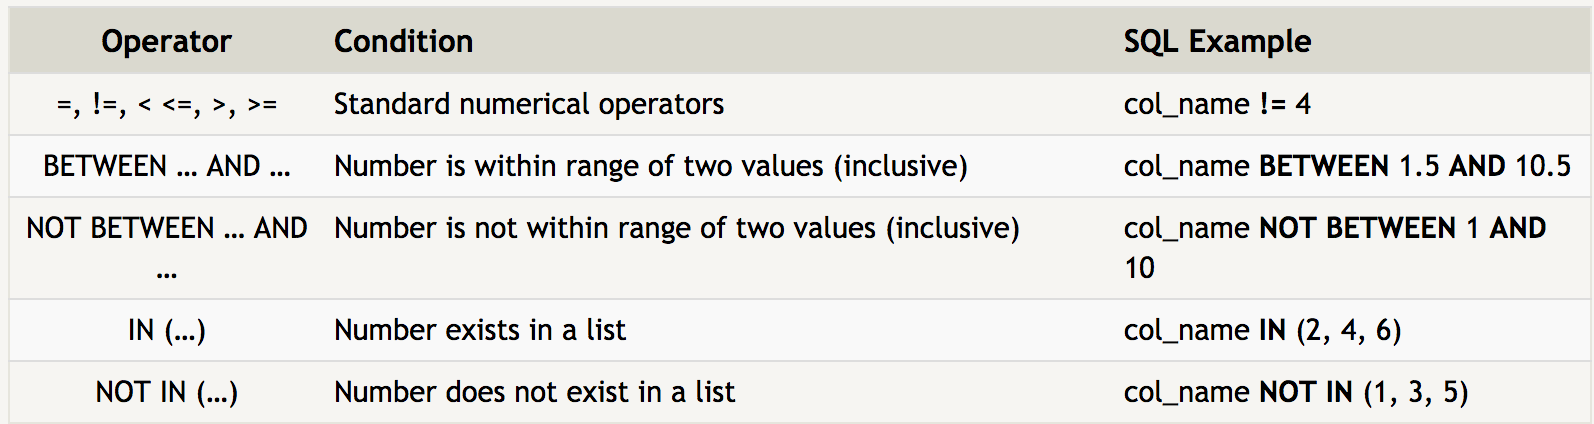
\includegraphics[width=14cm]{operators.png}
                \end{center}
            \end{figure}

    
            \begin{figure}[H]
                \begin{center}
                    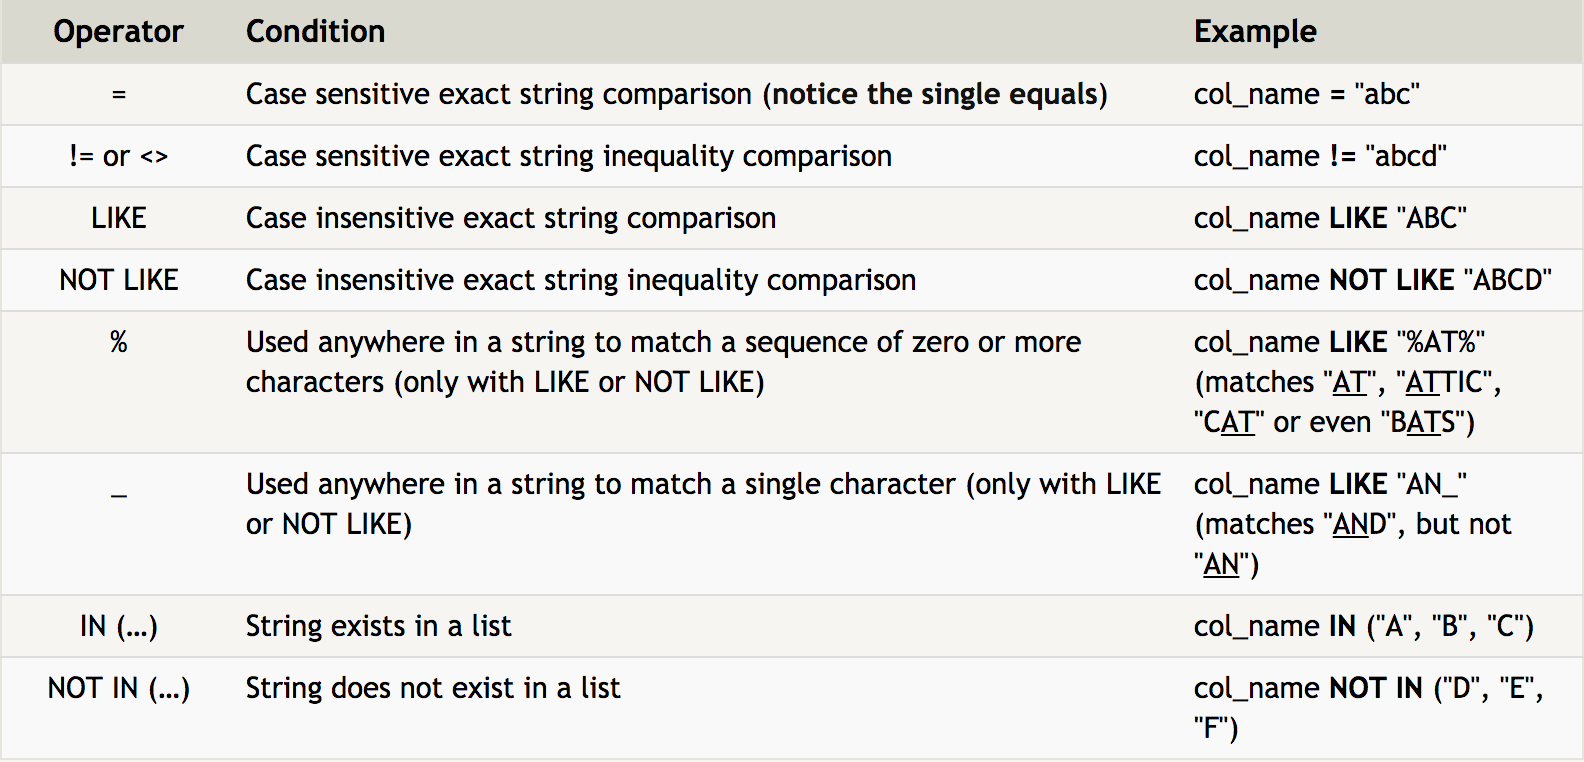
\includegraphics[width=14cm]{operators2.png}
                \end{center}
            \end{figure}

	Screenshots taken from SQLBolt! 
	


% Don't forget this line in order to increment the exercise counter
\nextexercice

%******************************************************************************%
%                                                                              %
%                             THE SQL PISCINE LOL                              %
%                                                                              %
%******************************************************************************%

\chapter{Day \exercicenumber: SLOWLY BECOMIN' POWERFUL IN SQL }
\extitle{SQL subqueries, GROUP BY, aggregate functions, HAVING}
\exfiles{04\_subquery.rb, 05\_aggregates.rb, 05a\_aggregates.rb}
\exnotes{Make sure to use docker cp to store your files on the host computer, then add it to a git repo after!}
\makeheaderfiles

	Look at this example! \\
    
            \begin{figure}[H]
                \begin{center}
                    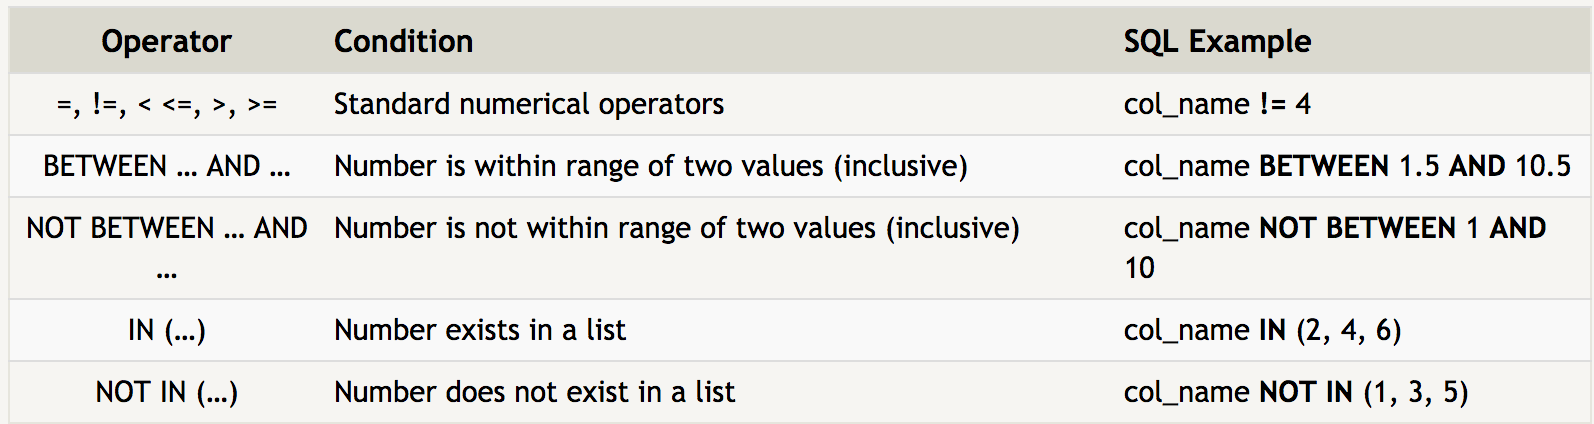
\includegraphics[width=14cm]{operators.png}
                \end{center}
            \end{figure}

	\begin{itemize}\itemsep1pt 
		\item Subqueries are easy, aren't they? It's just a query inside of another query! 
			However, think about the type of subquery: is it correlated? A correlated 
			subquery is where the subquery is dependent on a column from the outer query, 
			meaning it runs repeatedly. 
		\item GROUP BY groups the same column results together, allowing you to use aggregate functions. 
			What happens when you use GROUP BY on more than one column? 
		\item HAVING is just like WHERE, but it happens after the GROUP BY rather than before. 
			We'll get to SQL's logical order 
			later, for now-- just know that SQL's syntactical order isn't its logical order. 
		\item Aggregate functions are helpful functions you can use on groups! What are some of the most 
			commonly used ones?
	\end{itemize}

            \begin{figure}[H]
                \begin{center}
                    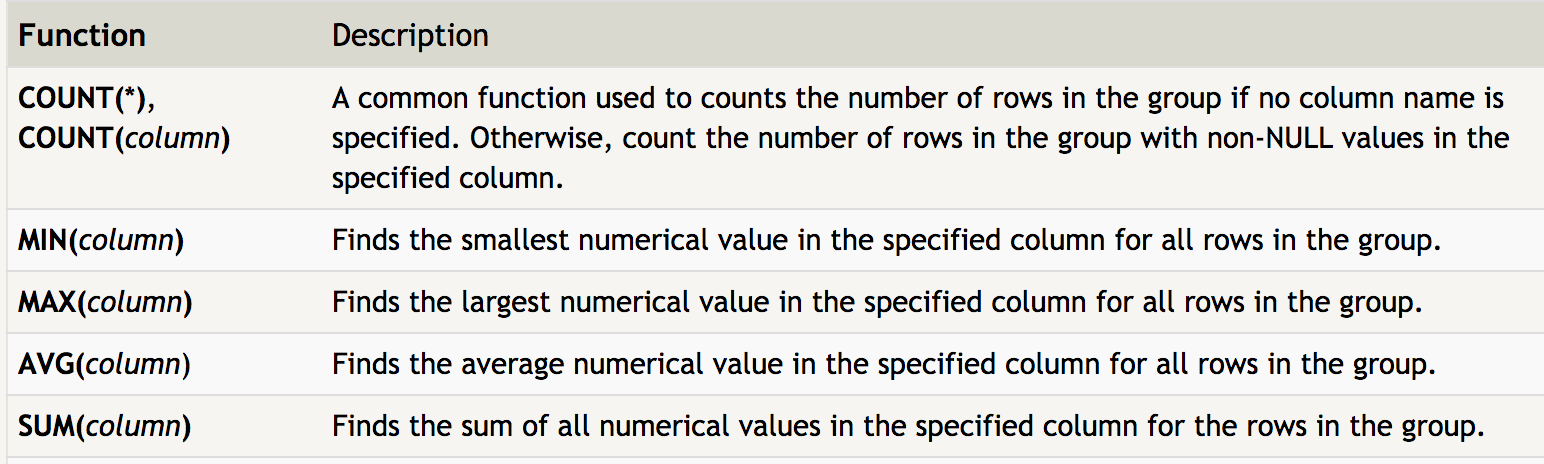
\includegraphics[width=14cm]{aggregate_functions.png}
                \end{center}
            \end{figure}

	   Another chart from SQLBolt!

% Don't forget this line in order to increment the exercise counter
\nextexercice

%******************************************************************************%
%                                                                              %
%                             THE SQL PISCINE LOL                              %
%                                                                              %
%******************************************************************************%

\chapter{Day \exercicenumber: YOUR POWER LEVEL IS RISING. }

\extitle{SQL JOINS, ORDER BY, LIMIT, join tables, primary key, foreign key, DB schema}
\exfiles{06\_joins.rb, 07\_joins.rb, 07a\_joins.rb}
\exnotes{Make sure to use docker cp to store your files on the host computer, then add it to a git repo after!}
\makeheaderfiles


	Look at this example! \\
    
            \begin{figure}[H]
                \begin{center}
                    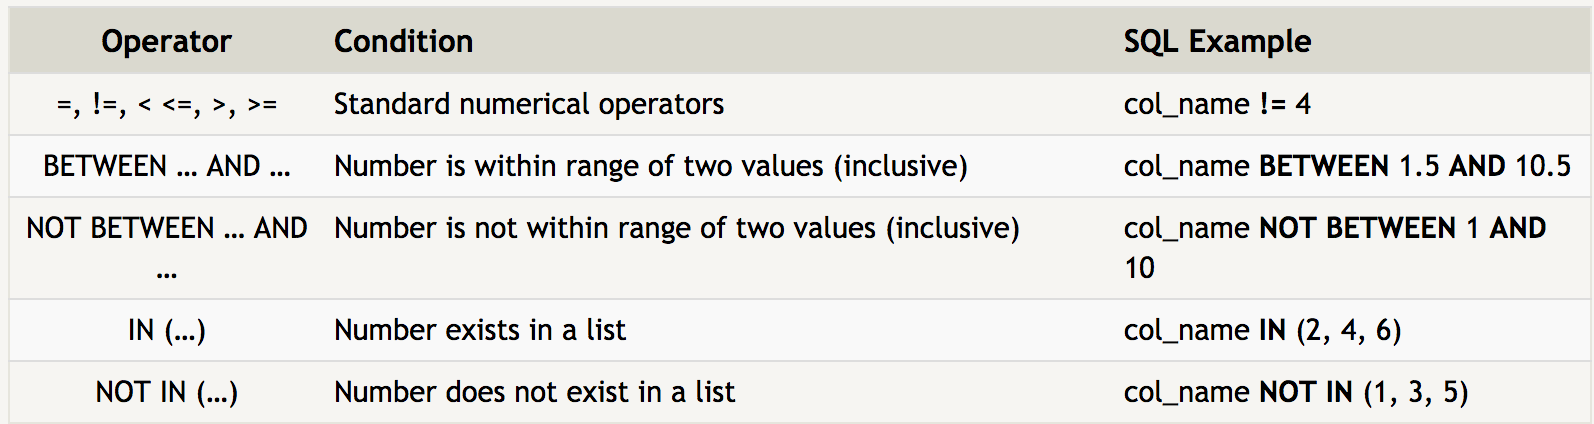
\includegraphics[width=14cm]{operators.png}
                \end{center}
            \end{figure}

	\begin{itemize}\itemsep1pt 
		\item What does a JOINS do? It combines rows from two or more tables together! 
		\item ORDER BY orders your results based on some specific column, with options ASC or DESC
		\item LIMIT simply limits the amount of results you'll get back to a certain number
		\item A schema is basically just a view of the entire database 
		\item Primary keys are used to uniquely identify each row in the table. 
		\item Foreign keys are used to join two tables together!
		\item If an employees table has a boss\_id foreign key, employees will belong to boss while boss will have 
			many employees. 
		\item A join table is needed to deal with a many-to-many relationship! Think about it for a lil' bit. 
			Why is a join table needed? 
	\end{itemize}

	Rather than posting an image of what happens on a regular join, here is a link to a \href{https://blog.codinghorror.com/a-visual-explanation-of-sql-joins/}{visual representation 
	of SQL joins}.
% Don't forget this line in order to increment the exercise counter
\nextexercice

%******************************************************************************%
%                                                                              %
%                             THE SQL PISCINE LOL                              %
%                                                                              %
%******************************************************************************%

\chapter{Day \exercicenumber: AND THIS IS TO GO FURTHER BEYOND }

\extitle{SQL IS NULL/NOT NULL, OUTER JOINS, COALESCE, CASE, self joins, ternary logic}
\exfiles{08\_null.rb, 09\_self\_joins.rb, wrapper program}
\exnotes{Make sure to use docker cp to store your files on the host computer, then add it to a git repo after!}
\makeheaderfiles

	Look at this example! \\
    
            \begin{figure}[H]
                \begin{center}
                    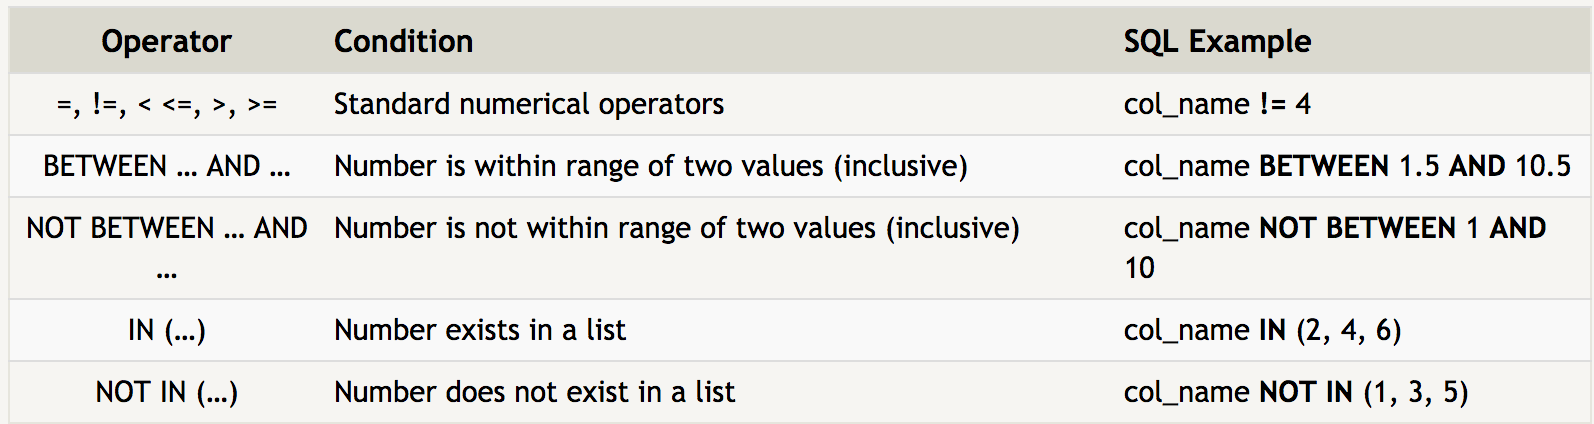
\includegraphics[width=14cm]{operators.png}
                \end{center}
            \end{figure}

	\begin{itemize}\itemsep1pt 
		\item Why do you have to use IS NULL/IS NOT NULL instead of just = or != NULL? 
			Recall that NULL is unknown, so if you compare NULL = NULL, you get false 
			since they're both unknown. 
		\item Outer joins! Look above to the visual representation of SQL joins. Think about 
			why outer joins can result in NULLs. 
		\item CASE statement is self explanatory
		\item COALESCE is used to fill out NULL values with default ones!   
		\item In what cases would you use self joins and why?  
		\item What is SQL's ternary logic? -> True, false, null
	\end{itemize}

	Look at this example of a basic wrapper program! \\ 

	\begin{figure}[H]
		\begin{center}
			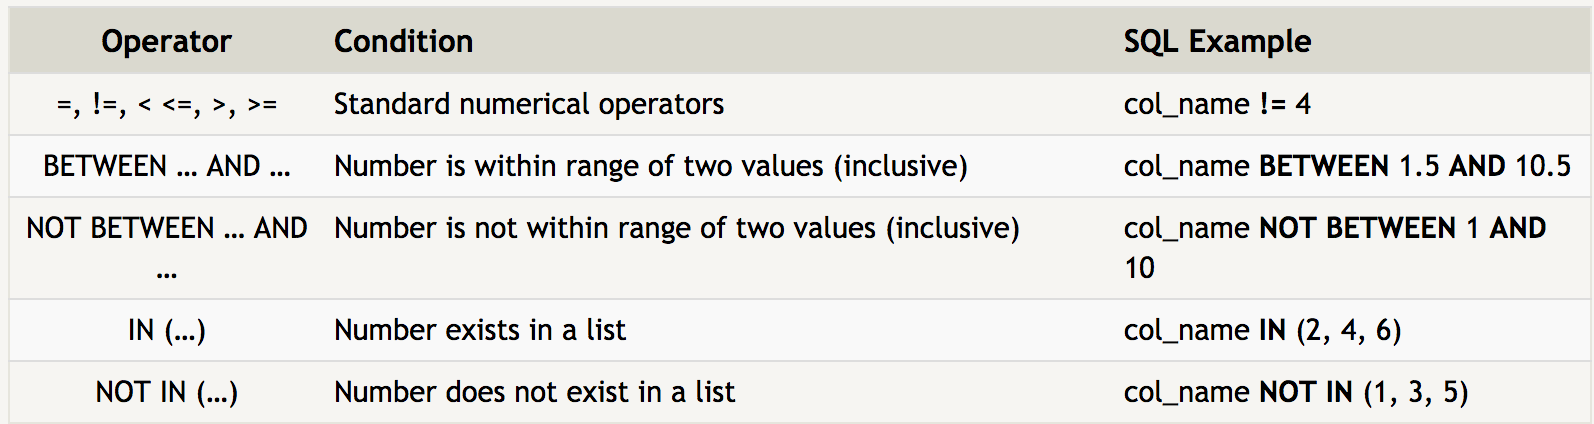
\includegraphics[width=14cm]{operators.png}
		\end{center}
	\end{figure}

% Don't forget this line in order to increment the exercise counter
\nextexercice


%******************************************************************************%
%                                                                              %
%                                 Bonus part                                   %
%                                                                              %
%******************************************************************************%
\chapter{Bonus part}

	Whoa, I can't believe you actually finished everything. You cheated, didn't you?! 
	Well, whatever. Now, it's time for bonuses! Well, there's really only one 
	plausible bonus for this project, so let's get right to it. \\ 

	Your bonus will be creating 10 additional queries for information you want 
	to get from the database! Write these 10 queries in a separate file, 
	then make a skeleton and spec file for said queries. After that, challenge 
	your peers to solve said queries! You will get the bonus points provided 
	none of your peers can solve all 10 queries that you've created. \\ 

	If your material is good, it'll be added to the curriculum to make the 
	next gen of H2S SQL students suffer! 

%******************************************************************************%
%                                                                              %
%                           Turn-in and peer-evaluation                        %
%                                                                              %
%******************************************************************************%
\chapter{Turn-in and peer-evaluation}
    Turn your work in using your \texttt{GiT} repository, as
    usual. Only work present on your repository will be graded in defense. \\
	
	Remember to store all your work on a git repository-- make sure to add, commit, then push! \\ 

    Good luck and don't forget to "cd (where you stored your work) \&\& rm -rf *" once you're done.

    . \\

    . \\

    . \\ 

    . \\ 

    . \\ 

    . \\

    . \\

    . \\

    . \\
    
    . \\

    . \\
    
    . \\

    . \\

    If you've actually followed instructions and stored your work, you'll be fine.

%******************************************************************************%
\end{document}
